\documentclass[journal]{IEEEtran}
\usepackage{amsmath,amssymb,amsfonts}
\usepackage{algorithmic}
\usepackage{array}
\usepackage[caption=false,font=normalsize,labelfont=sf,textfont=sf]{subfig}
\usepackage{textcomp}
\usepackage{stfloats}
\usepackage{url}
\usepackage{verbatim}
\usepackage{graphicx}
\usepackage{mathtools}
\usepackage{bm}
\usepackage{array}
\usepackage{subcaption} % Provides the subfigure environment for side-by-side figures
\usepackage{ragged2e} % For text alignment
\usepackage{caption}  % For captions
\usepackage[linesnumbered,ruled,vlined]{algorithm2e}
\usepackage{xcolor}  
\usepackage[hidelinks]{hyperref}

\newcommand{\bfit}[1]{\textbf{\textit{#1}}} % Bold and italic text
\newcommand{\fixspace}{\vspace{-0.9\baselineskip}} % Reduce space between sections

\hyphenation{op-tical net-works semi-conduc-tor IEEE-Xplore}
\def\BibTeX{{\rm B\kern-.05em{\sc i\kern-.025em b}\kern-.08em
    T\kern-.1667em\lower.7ex\hbox{E}\kern-.125emX}}
\usepackage{balance}

\bibliographystyle{IEEEtran}

\begin{document}
\title{\textbf{A Brief Review of the Chan--Vese Paper}: \\ \textit{Active Contours Without Edges}}
\author{\href{https://github.com/CamiloMartinezM}{Camilo A. Martínez M.}, \textit{Universität des Saarlandes} \\
    \vspace*{0.5\baselineskip} \today \vspace*{-\baselineskip}
    \thanks{This document template was developed by the IEEE Publication Technology Department, distributed under the \LaTeX \ Project Public License (LPPL) ( http://www.latex-project.org/ ) version 1.3. A copy of the LPPL, version 1.3, is included in the base \LaTeX \ documentation of all distributions of \LaTeX \ released 2003/12/01 or later. The opinions expressed here are entirely that of the author. No warranty is expressed or implied.}}

\maketitle

\begin{abstract}
    This report presents a brief review of the Chan--Vese model proposed in the paper \emph{Active Contours Without Edges} by T. Chan and L. Vese \cite{ChanVese}, published in 2001. This paper introduced a new model for image segmentation based on the \emph{Mumford--Shah functional} using a powerful mathematical backbone, the level set method \cite{Osher1988}. This report provides an overview of the prior works that led to the findings of Chan and Vese, the formulation of the Chan--Vese model, the energy minimization and discretization, its limitations, as well as some qualitative results obtained by the authors. Furthermore, some of the extensions and improvements to the model that came after the publication of the original paper are briefly touched upon. Finally, the report concludes with a discussion of the impact the paper had on future research, specifically in the field of image segmentation.
\end{abstract}

\begin{IEEEkeywords}
    IEEEtran, paper, journal, \textit{Active Contours Without Edges}, Chan--Vese, image segmentation, Mumford--Shah, level set method.
\end{IEEEkeywords}


\section{Introduction}
\IEEEPARstart{T}{he} paper \emph{Active Contours Without Edges} by Tony Chan and Luminita Vese \cite{ChanVese} is a seminal work in the field of image segmentation. It was published in 2001 and introduces a new model for image segmentation based on the \emph{Mumford--Shah functional} \cite{MumfordShah} using the level set method, proposed by Osher and Sethian \cite{Osher1988} in 1988, as the mathematical backbone. The paper has been cited over 8,000 times according to IEEEXplore\textsuperscript{\textregistered} and has had a significant impact on the field of \emph{Computer Vision}, particularly in the topic of image segmentation, one of its most widely studied problems. Over the years, it has found an application in medical imaging, robotics, video surveillance, materials science, autonomous driving, and many others.

\subsection{Prior Works}
\noindent Before the Chan--Vese model, some early methods existed for image segmentation, namely, thresholding, region growing, and edge-based segmentation. Some improvements were made with the introduction of the \emph{snakes} and \emph{active contours} models by Kass et al. \cite{Kass1988}. Nevertheless, the challenge of segmenting images without clear edges remained. Table~\ref{tab1:key-papers} shows a list of some of the prior founding works that led to the development of the Chan--Vese model.

\begin{table}[h]
    \begin{center}
        \caption{Prior Works to the Chan--Vese Model}
        \label{tab1:key-papers}
        \begin{tabular}{| p{0.225\textwidth} c c |}
            \hline
            \textbf{Title}                                                  & \textbf{Authors}       & \textbf{Year} \\
            \hline
            Boundary detection by minimizing functionals \cite{MumfordShah} & D. Mumford and J. Shah & 1985          \\
            \hline
            Snakes: Active contour models \cite{Kass1988}                   & M. Kass et al.         & 1988          \\
            \hline
            A topology independent shape modeling scheme \cite{Malladi1993} & R. Malladi et al.      & 1993          \\
            \hline
            On geodesic active contours \cite{Caselles}                     & V. Caselles et al.     & 1997          \\
            \hline
        \end{tabular}
    \end{center}
\end{table}

\section{The Chan--Vese Model}

\subsection{The ``Fitting'' Problem}
T. Chan and L. Vese (2001) proposed a specific region-based active contour model, where the image is segmented into \textbf{two phases/regions}: object and background. A summary of the mathematical derivation of the model is presented below.

Assume we have an image \( u({\bm{x}}), \bm{x} \in \Omega \), and the image is formed by two regions with mean intensity values: \( u_{in} \) and \( u_{out} \). Our \textit{evolving} boundary curve \( C \) separates the two regions. Then, we can define a \emph{fitting} term that penalizes deviations from the mean intensity values:
\begin{equation}\label{eq:fitting}
    \textrm{fitting}(C) \coloneq F_{in}(C) + F_{out}(C)
\end{equation}

Furthermore, using a Mean-Squared Error (MSE) approach, equation \eqref{eq:fitting} can be developed as:
\begin{align*}
    \textrm{fitting}(C) & = \phantom{\int\limits_{inside(C)}} F_{in}(C) \phantom{\int\limits_{out(C)}} \color{black}{+} \phantom{\int\limits_{in(C)}} F_{out}(C) \phantom{\int\limits_{out(C)}}                                                                                                              \\
                        & = \underbrace{\int\limits_{\scriptstyle in(C)} |u(\bm{x}) - c_{in}|^2 \, d\bm{x}}_{\text{$> 0$, if $u(\bm{x})$ deviates from $c_{in}$}} + \underbrace{\int\limits_{\scriptstyle out(C)} |u(\bm{x}) - c_{out}|^2 \, d\bm{x}}_{\text{$> 0$, if $u(\bm{x})$ deviates from $c_{out}$}}
\end{align*}

Thus, the minimizer $C_0$ that satisfies \(\textrm{fitting}(C_0) \approx 0\), which is the contour that segments the image into the two regions with mean intensity values \(c_{in}\) and \(c_{out}\), can be defined as:
\begin{equation}\label{eq:minimization}
    C_0 = \inf_C \{\textrm{fitting(C)}\} = \inf_C \{F_{in}(C) + F_{out}(C)\}
\end{equation}
Figure \ref{tab2:fitting-problem} shows the different cases of the fitting term for different contours \( C \) that enclose the object in the image. The objective $C_0$ is the one that perfectly encloses the object, i.e., $fitting(C_0) = 0$, as shown in the lower-right example.

\subsection{Formulation as an Energy Functional}
Now, we can introduce the energy functional \( F(C) \) as:

\begin{equation}\label{eq:energy-functional-simplified}
    F(C) = \underbrace{\mu \cdot \textrm{Length}(C) + \nu \cdot \textrm{Area}(\textrm{in}(C))}_{\text{penalize the "size" of $C$}} + \textrm{fitting}(C)
\end{equation}

\begin{figure}[!t]
    \centering
    \begin{tabular}{@{}>{\centering\arraybackslash} m{0.25\textwidth} @{} >{\centering\arraybackslash} m{0.25\textwidth} @{}}
        \small $F_{in}(C) > 0, F_{out}(C) \approx 0$, \, \, fitting $> 0$                                                    & \small $F_{in}(C) \approx 0, F_{out}(C) > 0$, \, \, fitting $> 0$                                                     \\
        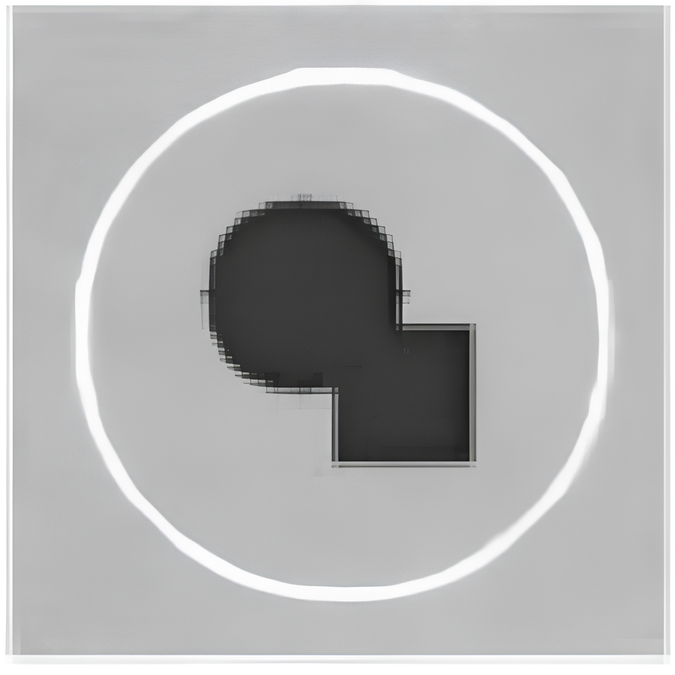
\includegraphics[width=0.25\textwidth,height=0.25\textheight,keepaspectratio]{images/fitting-problem-upper-left.png} & 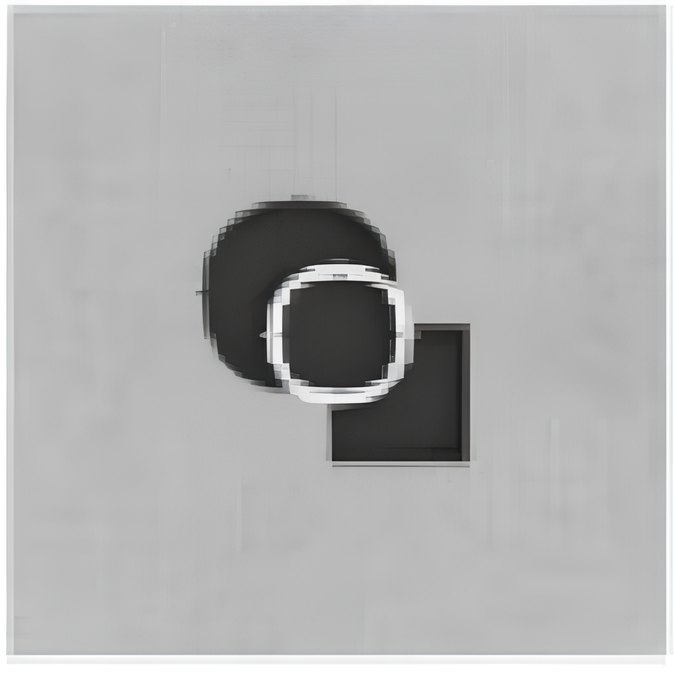
\includegraphics[width=0.25\textwidth,height=0.25\textheight,keepaspectratio]{images/fitting-problem-upper-right.png} \\
        \small $F_{in}(C) > 0, F_{out}(C) > 0$, \, \, fitting $> 0$                                                          & \small $F_{in}(C) \approx 0, F_{out}(C) \approx 0$, \, \, fitting $= 0$                                               \\
        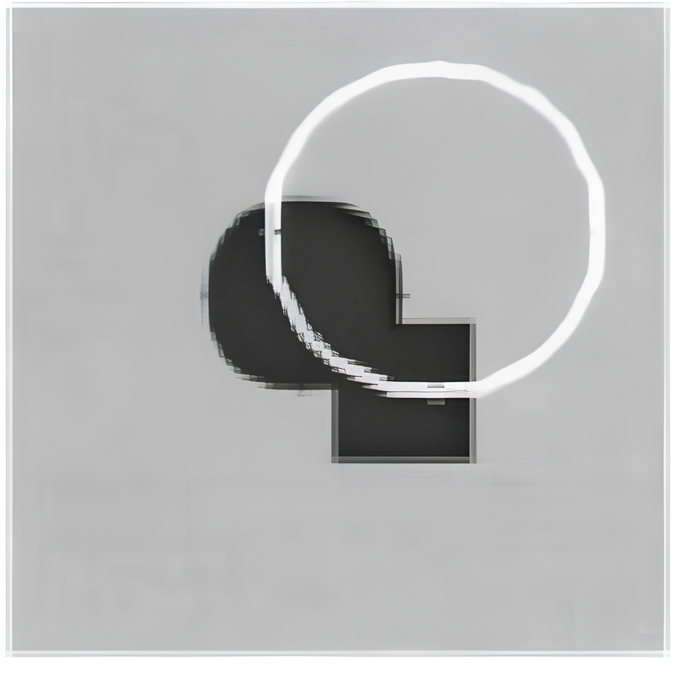
\includegraphics[width=0.25\textwidth,height=0.25\textheight,keepaspectratio]{images/fitting-problem-lower-left.png} & 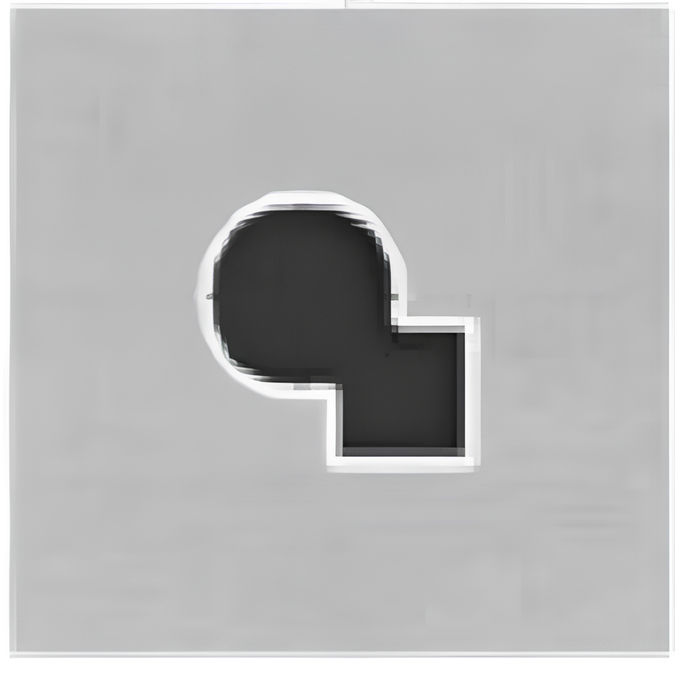
\includegraphics[width=0.25\textwidth,height=0.25\textheight,keepaspectratio]{images/fitting-problem-lower-right.png} \\
    \end{tabular}
    \caption{Consider all possible cases of $C$ enclosing the object in the image. The \emph{fitting} term is minimized only in the case when $C$ is exactly on the boundary of the object \cite{ChanVese}.}
    \label{tab2:fitting-problem}
\end{figure}

\noindent Thus, the energy minimization problem becomes:
\begin{equation}
    C_0 = \inf_{C} F(C)
\end{equation}
\noindent with
\begin{equation}\label{eq:energy-functional}
    \begin{aligned}
        F(C) & = \mu \cdot \textrm{Length}(C) + \nu \cdot \textrm{Area}(\textrm{in}(C))                         \\
             & \quad + \lambda_1 \int\limits_{\scriptstyle in(C)} \left| u(\bm{x}) - c_{in} \right|^2 d\bm{x}   \\
             & \quad + \lambda_2 \int\limits_{\scriptstyle out(C)} \left| u(\bm{x}) - c_{out} \right|^2 d\bm{x}
    \end{aligned}
\end{equation}
\noindent where $\mu, \, \nu \in \mathbb{R}_0^+$, $\lambda_1, \lambda_2 \in \mathbb{R}^+$ are fixed parameters.
This can be formulated and solved using the \textbf{level set method} \cite{Osher1988}, as presented in Sec.~\ref{sec:level-set-formulation}.

\subsection{Comparison with the Mumford--Shah Model}
The \emph{Mumford--Shah model} introduced in 1985 \cite{MumfordShah} by D. Mumford and J. Shah is defined as \cite{Pascal2023}:
\[
    E_{MS}(K, u) = \int_{\Omega} (f - u)^2 \, dx + \gamma \int_{\Omega \backslash K} |\nabla u|^2 \, dx + \lambda |K|
\]
This model leads to the \textbf{Chan--Vese} approach
\begin{itemize}
    \item if we have piecewise constant approximations $u$, i.e., $u = \text{constant } c_i$ on each connected component $R_i$ of $\Omega \setminus C$.
    \item and an edge set $K$ that separates $\Omega$ into \textit{two phases}.
\end{itemize}
This reduced case is called the \emph{minimal partition problem} \cite{ChanVese}.

\subsection{The Level-Set Formulation}\label{sec:level-set-formulation}
In the level set method \cite{Osher1988}, $C \subset \Omega$ is represented by the zero level set of a \emph{Lipschitz function} $\phi: \Omega \rightarrow \mathbb{R}$, such that
\[
    \begin{cases}
        C = \partial \omega = \{ (x, y) \in \Omega : \phi(x, y) = 0 \},     \\
        \textrm{in(C)} = \omega = \{ (x, y) \in \Omega : \phi(x, y) > 0 \}, \\
        \textrm{out(C)} = \Omega \setminus \bar{\omega} = \{ (x, y) \in \Omega : \phi(x, y) < 0 \}.
    \end{cases}
\]
Intuitively, this \bfit{Lipschitz function} $\phi$ is by definition limited in how fast it can change: there exists a real number such that, for every pair of points on the graph of this function, the absolute value of the slope of the line connecting them is not greater than a real number called the \bfit{Lipschitz constant} of the function, $L$ \cite{wiki:LipschitzContinuity}. See figure \ref{fig:phi} for an illustration of how $C$ and $\phi$ are related to each other.

Now, our aim is to compute the \emph{Euler-Lagrange} equation associated with the introduced energy functional $F(C)$ of equation \eqref{eq:energy-functional-simplified} by replacing the unknown variable $C$ by the new variable $\phi$ \cite{Zhao1996}.

\begin{figure}[!t]
    \centering
    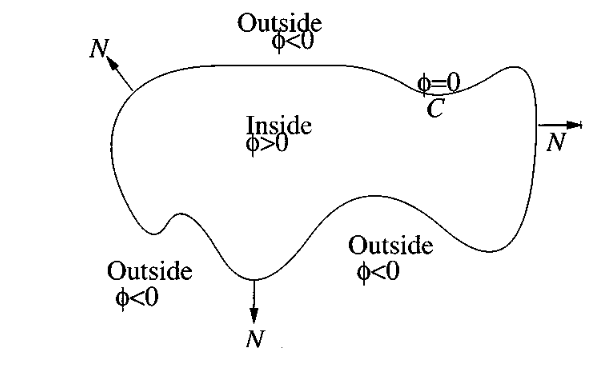
\includegraphics[width=0.5\textwidth]{images/phi.png}
    \caption{Illustration of the relationship between $C$ and $\phi$; Curve $C = \{ (x, y) : \phi(x, y) = 0 \}$ propagating in normal direction \cite{ChanVese}.}
    \label{fig:phi}
\end{figure}

On the other hand, we can define the \emph{Heaviside} function $H(z)$ and the \emph{Dirac delta} function $\delta_0(z)$ as:
\[
    H(z) = \begin{cases}
        0, & \text{if } z < 0    \\
        1, & \text{if } z \geq 0
    \end{cases}, \,
    \delta_0(z) = \frac{d}{dz} H(z) = \begin{cases}
        \infty, & \text{if } z = 0,   \\
        0,      & \text{if } z \neq 0
    \end{cases}
\]

These functions, when applied to $\phi$, allow us to compute the \emph{length} and \emph{area} of the curve $C$, as defined below and illustrated in figure \ref{fig:heaviside-phi-illustration}:
\small
\begin{equation}\label{eq:length-area}
    \textrm{Length}\{\phi = 0\} = \int_{\Omega} |\nabla H(\phi(\bm{x}))| \, d\bm{x} = \int_{\Omega} \delta_0(\phi(\bm{x})) |\nabla \phi(\bm{x})| \, d\bm{x}
\end{equation}
\begin{equation}\label{eq:area}
    \textrm{Area}\{\phi \geq 0\} = \int_{\Omega} H(\phi(\bm{x})) \, d\bm{x}
\end{equation}
\normalsize

\begin{figure}[!t]
    \centering
    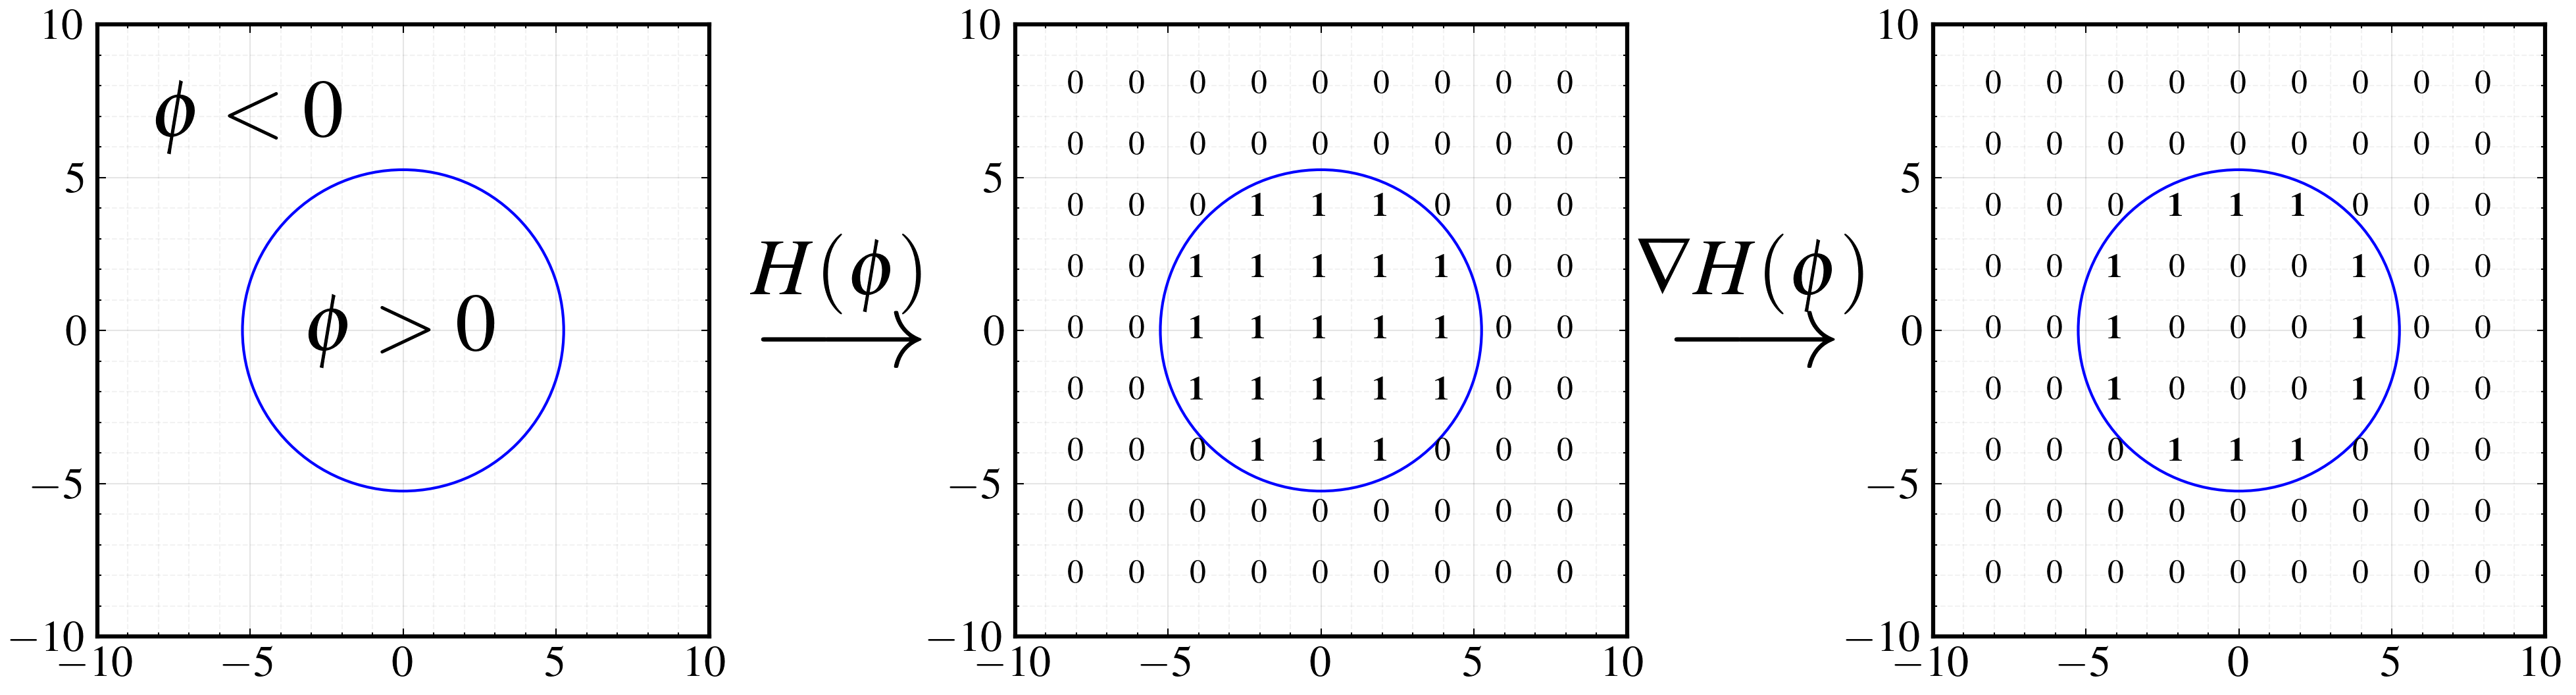
\includegraphics[width=0.5\textwidth,keepaspectratio]{images/heaviside-and-phi-illustration.png}
    \caption{From \textbf{left} to \textbf{right}, the process of applying $H$ to $\phi$ and then taking the gradient.}
    \label{fig:heaviside-phi-illustration}
\end{figure}

Thus, using equations \ref{eq:length-area} and \eqref{eq:area} in \eqref{eq:energy-functional}, we can rewrite the energy functional $F(C)$ as:
\begin{align*}
    F(\phi)
     & = \mu \underbrace{\int_{\Omega} \delta(\phi(\bm{x})) |\nabla \phi(\bm{x})| \, d\bm{x}}_{\textrm{Length(C)}} + \nu \underbrace{\int_{\Omega} H(\phi(\bm{x})) \, d\bm{x}}_{\textrm{Area(in(C))}}      \\
     & \quad + \lambda_1 \underbrace{\int_{\Omega} |u(\bm{x}) - c_{in}|^2 H(\phi(\bm{x})) \, d\bm{x}}_{\text{$= $$\int\limits_{\scriptstyle in(C)} \left| u(\bm{x}) - c_{in} \right|^2 d\bm{x}$}}          \\
     & \quad + \lambda_2 \underbrace{\int_{\Omega} |u(\bm{x}) - c_{out}|^2 (1 - H(\phi(\bm{x}))) \, d\bm{x}}_{\text{$= $$\int\limits_{\scriptstyle out(C)} \left| u(\bm{x}) - c_{out} \right|^2 d\bm{x}$}} \\
\end{align*}
In practice, $H$ and $\delta_0$ are approximated by \emph{continuous functions} $H_{\epsilon}$ and $\delta_{\epsilon}$, respectively, such that $H_\epsilon$ is at least $C^2(\bar{\Omega})$ and $\lim\limits_{\epsilon \to 0} H_{\epsilon}(z) = H(z)$ and $\lim\limits_{\epsilon \to 0} \delta_{\epsilon}(z) = \delta_0(z)$. The regularized functions analyzed by the authors are shown in figure \ref{fig:heaviside-regularized} and further explained in Sec. \ref{sec:parameter-selection}.

\begin{figure}[!t]
    \centering
    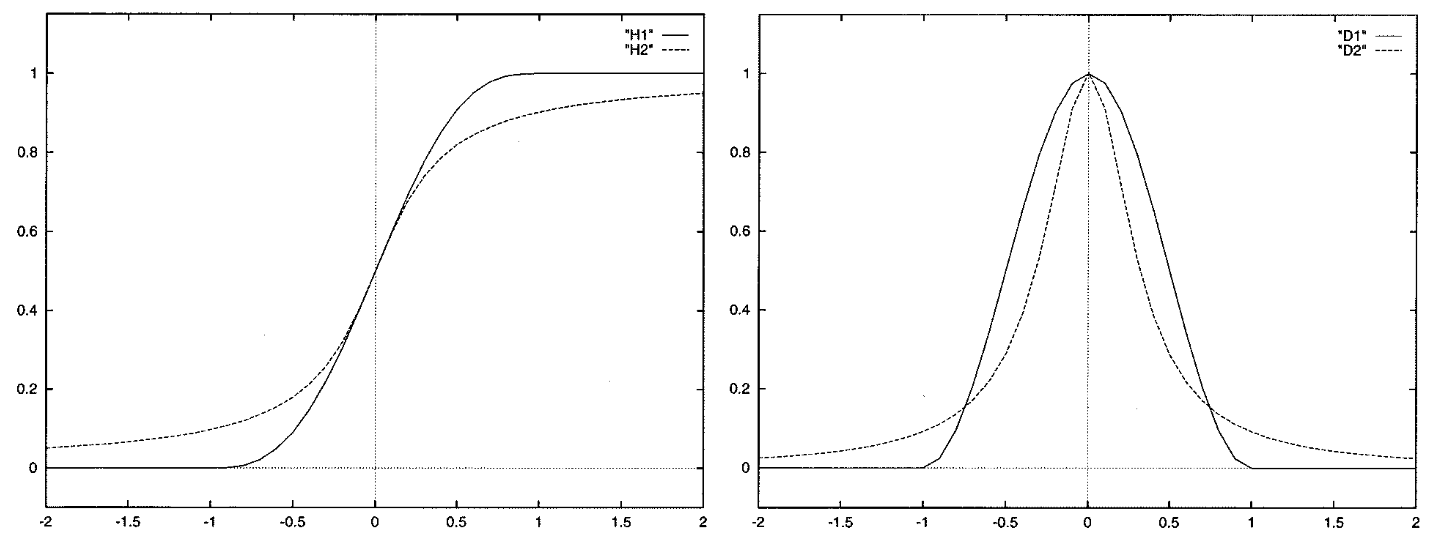
\includegraphics[width=0.5\textwidth]{images/heaviside-regularized.png}
    \caption{Two different regularizations of the (left) heaviside function $H$ and (right) delta function $\delta_0$ \cite{ChanVese}.}
    \label{fig:heaviside-regularized}
\end{figure}

Finally, our \emph{regularized} energy functional $F_\epsilon(\phi)$ is given by:
\begin{align*}
    F(\phi)
     & = \mu \int_{\Omega} \delta_\epsilon(\phi(\bm{x})) |\nabla \phi(\bm{x})| \, d\bm{x} + \nu \int_{\Omega} H_\epsilon(\phi(\bm{x})) \, d\bm{x} \\
     & \quad + \lambda_1 \int_{\Omega} |u(\bm{x}) - c_{in}|^2 H_\epsilon(\phi(\bm{x})) \, d\bm{x}                                                 \\
     & \quad + \lambda_2 \int_{\Omega} |u(\bm{x}) - c_{out}|^2 (1 - H_\epsilon(\phi(\bm{x}))) \, d\bm{x}                                          \\
\end{align*}

\subsection{Energy Minimization \& Discretization}
The \emph{Euler--Lagrange equation} for an energy functional of the form is given by the following expression:
\[
    E(\phi) = \int_{\Omega} F(x, y, \phi, \phi_x, \phi_y) \, d\bm{x} \Longrightarrow F_\phi - \partial_x F_{\phi_x} - \partial_y F_{\phi_y} = 0
\]
with \textit{natural boundary conditions}
\[
    \bm{n}^\top \left( \begin{array}{c}
            F_{\phi_x} \\
            F_{\phi_y}
        \end{array} \right) = 0
\]
where $\bm{n}$ denotes a normal vector to the image boundary $\partial \Omega$.

In our case study, remembering that we are keeping $c_{in}$ and $c_{out}$ fixed, and minimizing $F_{\epsilon}$ with respect to $\phi$, we deduce the associated \emph{Euler--Lagrange} equation for $\phi$:
\[
    \begin{cases}
        F_\phi     & = \nu \delta_\epsilon(\phi) + \lambda_1 |u - c_{in}|^2 \delta_\epsilon(\phi) - \lambda_2 |u - c_{out}|^2 \delta_\epsilon(\phi), \\
        F_{\phi_x} & = 2 \mu \delta_\epsilon(\phi) \phi_x,                                                                                           \\
        F_{\phi_y} & = 2 \mu \delta_\epsilon(\phi) \phi_y                                                                                            \\
    \end{cases}
\]
\vspace{-0.5\baselineskip}

Thus, for $t \geq 0$, we get:
\begin{equation}\label{eq:phi-pde}
    \begin{aligned}
        \frac{\partial \phi}{\partial t} & = \delta_{\epsilon}(\phi) \left[ \mu \, \textrm{div} \left( \frac{\nabla \phi}{|\nabla \phi|} \right) - \nu - \lambda_1 (u - c_{in})^2 + \lambda_2 (u - c_{out})^2 \right] \\
                                         & = 0 \quad \textrm{in} \quad (0, \infty) \times \Omega
    \end{aligned}
\end{equation}
With initial contour $\phi(0, x, y) = \phi_0(x, y) \, \, \textrm{in} \, \, \Omega$ and boundary condition:
\begin{equation}\label{eq:boundary-condition}
    \frac{\delta_{\epsilon}(\phi)}{|\nabla \phi|} \frac{\partial \phi}{\partial \vec{n}} = 0 \quad \textrm{on} \quad \partial \Omega
\end{equation}
where $\vec{n}$ denotes the exterior normal to the boundary $\partial \Omega$, and $\partial \phi / \partial \vec{n}$ denotes the normal derivative of $\phi$ at the boundary.

To discretize and linearize the PDE given by \eqref{eq:phi-pde} in $\phi$, Chan and Vese (2001) used a \emph{finite differences implicit scheme}.

\small
\begin{align*}
    \frac{\phi_{i,j}^{n+1} - \phi_{i,j}^n}{\Delta t}
     & = \delta_h(\phi_{i,j}^n) \Bigg[ \frac{\mu}{h^2} \Delta_-^x                                                                                   \\
     & \quad \cdot \left(
    \frac{\Delta_+^x \phi_{i,j}^{n+1}}{\sqrt{(\Delta_+^x \phi_{i,j}^n)^2 / (h^2) + (\phi_{i,j+1}^n - \phi_{i,j-1}^n)^2 / (2h)^2}} \right)           \\
     & \quad + \frac{\mu}{h^2} \Delta_-^y \cdot \left(
    \frac{\Delta_+^y \phi_{i,j}^{n+1}}{\sqrt{\frac{(\phi_{i+1,j}^n - \phi_{i-1,j}^n)^2}{(2h)^2} + \frac{(\Delta_+^y \phi_{i,j}^n)^2}{h^2}}} \right) \\
     & \quad - \nu - \lambda_1 (u_{i,j} - c_1(\phi^n))^2 + \lambda_2 (u_{i,j} - c_2(\phi^n))^2 \Bigg]
\end{align*}
\normalsize

\section{Results}

\subsection{Parameter Selection}\label{sec:parameter-selection}
\begin{itemize}
    \item \( \lambda_1 = \lambda_2 = 1 \), \( \nu = 0 \), \( h = 1 \) (the step space), \( \Delta t = 0.1 \) (the time step).
    \item \( H_{2,\epsilon} \) and \( \delta_{2,\epsilon} \) were used with (\( \epsilon = h = 1 \)), in order to automatically detect \emph{interior contours}, and to ensure the computation of a \emph{global minimizer}. This is illustrated in figure \ref{fig:heaviside-regularized}, where \( H_{2,\epsilon} \) and \( \delta_{2,\epsilon} \) are shown to never reach zero, whereas \( H_{1,\epsilon} \) and \( \delta_{1,\epsilon} \) do. This means that the latter will not take into account global contributions, but only local ones, and thus will lead to a local minimizer of the energy \cite{ChanVese}.
    \item $\mu$ is \emph{experiment-dependent}, i.e. if our goal is to
          \begin{itemize}
              \item detect as many objects as possible $\Longrightarrow \text{small} \, \, \mu$.
              \item detect only larger objects $\Longrightarrow \text{large} \, \, \mu$.
          \end{itemize}
\end{itemize}

\subsection{Qualitative results}

Figure \ref{fig:noisy-detection} shows that the model works on a noisy synthetic image, with various shapes and an interior contour, which is automatically detected, without considering a second initial curve. Due to the level set implementation, the model allows an automatical change of topology, which is not affected by blurred boundaries or even lines not necessarily closed \cite{ChanVese}.

\begin{figure}[!t]
    \centering
    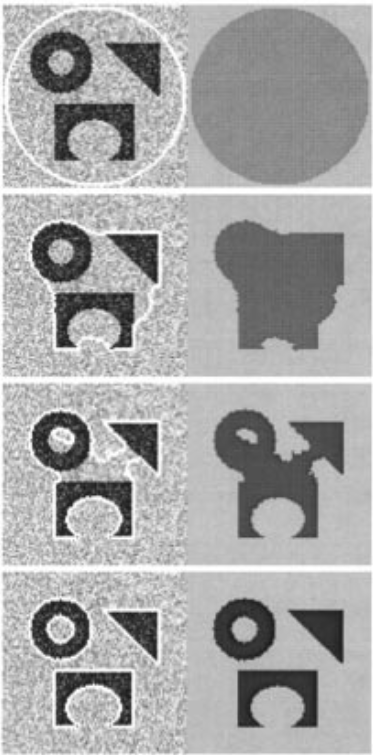
\includegraphics[width=0.24\textwidth,angle=90,origin=c]{images/results-noisy-detection.png}
    \vspace{-6\baselineskip}
    \caption{Detection of different objects from a noisy image, with various shapes and with an interior contour. \textbf{Bottom:} \( u \) and the contour. \textbf{Top:} the piecewise-constant approximation of \( u \). Size = \( 100 \times 100 \), \( \phi_0(x, y) = -\sqrt{(x - 50.5)^2 + (y - 50.5)^2} + 48.5 \), \( \mu = 0.1 \times 255^2 \), no reinitialization, cpu = 4.60 s \cite{ChanVese}.}
    \label{fig:noisy-detection}
\end{figure}
On the other hand, figure \ref{fig:kanizsa} shows an application of the model in detecting objects defined by a grouping according to Kanizsa's "proximity rule". This grouping can also be based on the chromatic resemblance or identity, among objects of the same shape or orientation \cite{ChanVese}. Refer to the Sec. \ref{sec:real-world-applications} for more qualitative results.

\begin{figure}[!t]
    \centering
    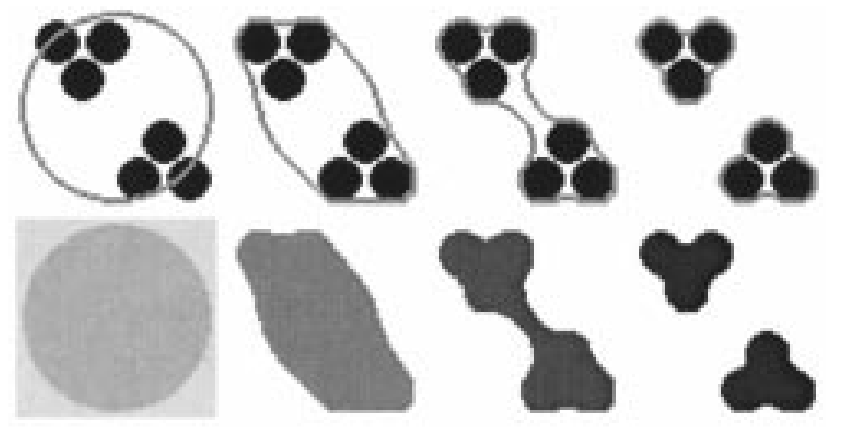
\includegraphics[width=0.5\textwidth,keepaspectratio]{images/results-kanizsa.png}
    \caption{Grouping based on Kanizsa's ``proximity rule.'' Size = \(64 \times 64\), \(\phi_0(x, y) = -\sqrt{(x - 32.5)^2 + (y - 32.5)^2} + 30\), \(\mu = 2 \cdot 255^2\), no reinitialization, cpu = 5.76 s \cite{ChanVese}.}
    \label{fig:kanizsa}
\end{figure}

\subsection{Limitations of the Model}\label{sec:limitations-of-the-model}
\begin{itemize}
    \item The Chan--Vese model is a specific case of the \emph{Mumford--Shah functional}, meaning it is limited to piecewise constant approximations of the image. Thus, it is not a general solution to the segmentation problem.
    \item There are objects which cannot be detected using the \emph{average intensity value} only, as illustrated in figure \ref{fig:limitations}.
\end{itemize}

\begin{figure}[!t]
    \centering
    \begin{minipage}{0.45\textwidth}
        \centering
        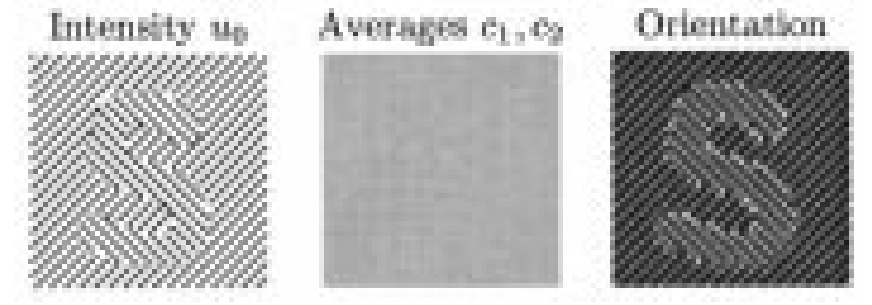
\includegraphics[width=\textwidth]{images/limitations-images.png}
    \end{minipage}
    \hfill
    \begin{minipage}{0.45\textwidth}
        \centering
        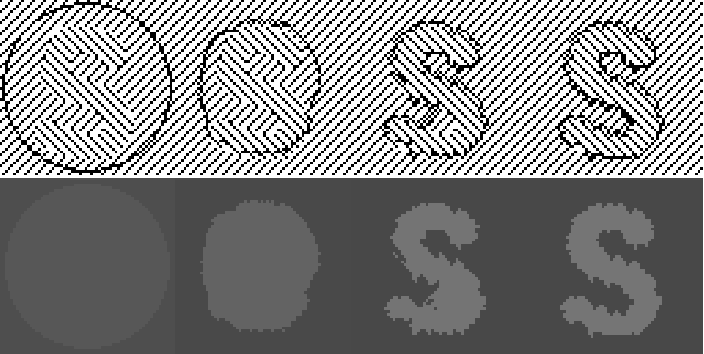
\includegraphics[width=\textwidth]{images/limitations.png}
    \end{minipage}
    \caption{Grouping based on orientation identity. The original image $u$ (\textbf{top}) is replaced by the orientation of the normal to the level curves of $u$. Size: $64 \times 64$, $\mu = 0.025 \cdot 255^2$, $\nu = 0.02 \cdot 255^2$, $\phi_0(x, y) = -\sqrt{(x - 32.5)^2 + (y - 32.5)^2} + 30$, five iterations of reinitialization, cpu = $10.25$ s \cite{ChanVese}.}
    \label{fig:limitations}
\end{figure}

\section{Impact on Research}

\subsection{Real-World Applications}\label{sec:real-world-applications}
Some of the real-world applications of the Chan--Vese model include: detection of minefields using reconnaissance aircraft images that identify many objects that are not mines; detection of Europe night-lights; detection of blurred contours of a galaxy, as shown in figure \ref{fig:galaxy-2}; and detection of a tumor in a MRI image, as shown in figure \ref{fig:mri} \cite{ChanVese}. It is important to point out that these results are not possible using classical snakes or active contours based on the gradient.

\begin{figure}[!t]
    \centering
    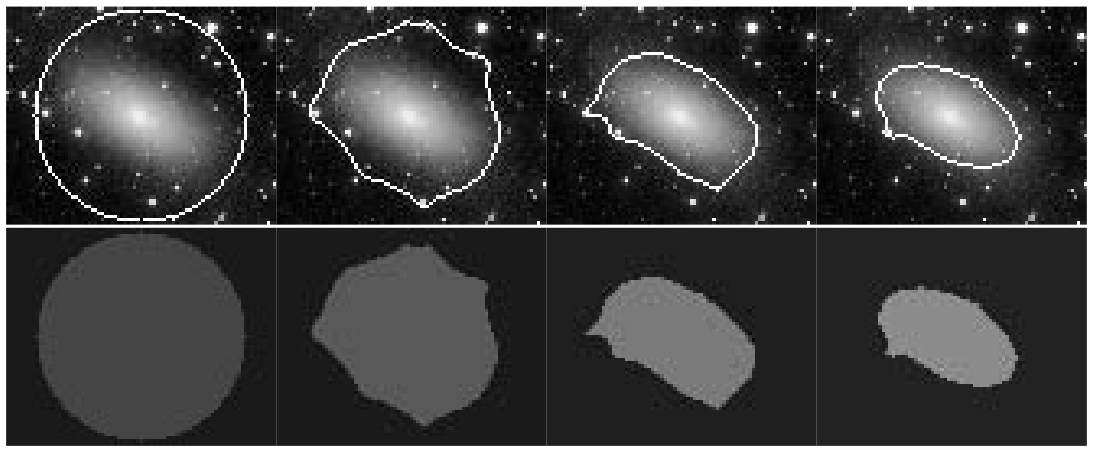
\includegraphics[width=0.5\textwidth,keepaspectratio]{images/results-galaxy-2.png}
    \caption{Detection of a galaxy with very smooth boundaries \cite{ChanVese}.}
    \label{fig:galaxy-2}
\end{figure}

\begin{figure}[!t]
    \centering
    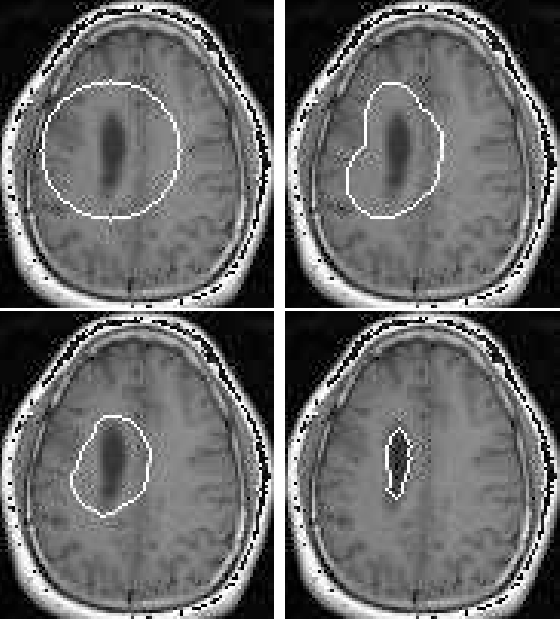
\includegraphics[height=0.275\textheight,width=0.45\textwidth]{images/results-mri.png}
    \caption{Detection of a tumor in a MRI image \cite{ChanVese}.}
    \label{fig:mri}
\end{figure}

\subsection{Extensions of the Chan-Vese Model}

% \begin{table}
%     \begin{center}
%         \caption{Summary of Key Papers.}
%         \label{tab2:derivative-papers}
%         \begin{tabular}{| p{0.225\textwidth} >{\centering}l >{\centering}c >{\centering}c |}
%             \hline
%             \textbf{Title}                                                                                          & \textbf{Last Author} & \textbf{Year} & \textbf{Citations} \tabularnewline
%             \hline
%             Level Set Method in Medical Imaging Segmentation                                                        & J. Suri              & 2019          & 12                 \tabularnewline
%             \hline
%             Efficient and robust segmentation and correction model for medical images                               & W. Jia               & 2018          & 3                  \tabularnewline
%             \hline
%             A two-stage image segmentation via global and local region active contours                              & Yugang Wang          & 2016          & 49                 \tabularnewline
%             \hline
%             Active contours driven by local likelihood image fitting energy for image segmentation                  & Qiang Chen           & 2015          & 94                 \tabularnewline
%             \hline
%             Robust image segmentation using local robust statistics and correntropy-based K-means clustering        & Li Zeng              & 2015          & 23                 \tabularnewline
%             \hline
%             An active contour model and its algorithms with local and global Gaussian distribution fitting energies & Yilun Wang           & 2014          & 86                 \tabularnewline
%             \hline
%             An efficient operator splitting method for local region Chan-Vese model                                 & Jun Liu              & 2013          & 2                  \tabularnewline
%             \hline
%         \end{tabular}
%     \end{center}
% \end{table}

Some modifications of the Chan--Vese model include \cite{Pascal2023}:
\begin{itemize}
    \item More sophisticated features than the grey value, such as colour channels, texture features, optic flow fields, etc.
    \item Additional statistical characterizations of a region, that is, not only mean, but also standard deviation, skewness, kurtosis, etc.
    \item A-priori knowledge, using a statistical characterization of the shapes to be expected.
\end{itemize}

All of these extensions have already been studied in the literature over the years. Some of the key papers are listed \textcolor{blue}{\href{https://www.connectedpapers.com/main/3bdcc6c663112ab10ffb5b5e875f8e2660cd5001/Active-contours-without-edges/derivative}{here}}, courtesy of \textcolor{blue}{\href{https://www.connectedpapers.com/}{@ConnectedPapers}}.

\begin{figure}[!t]
    \centering
    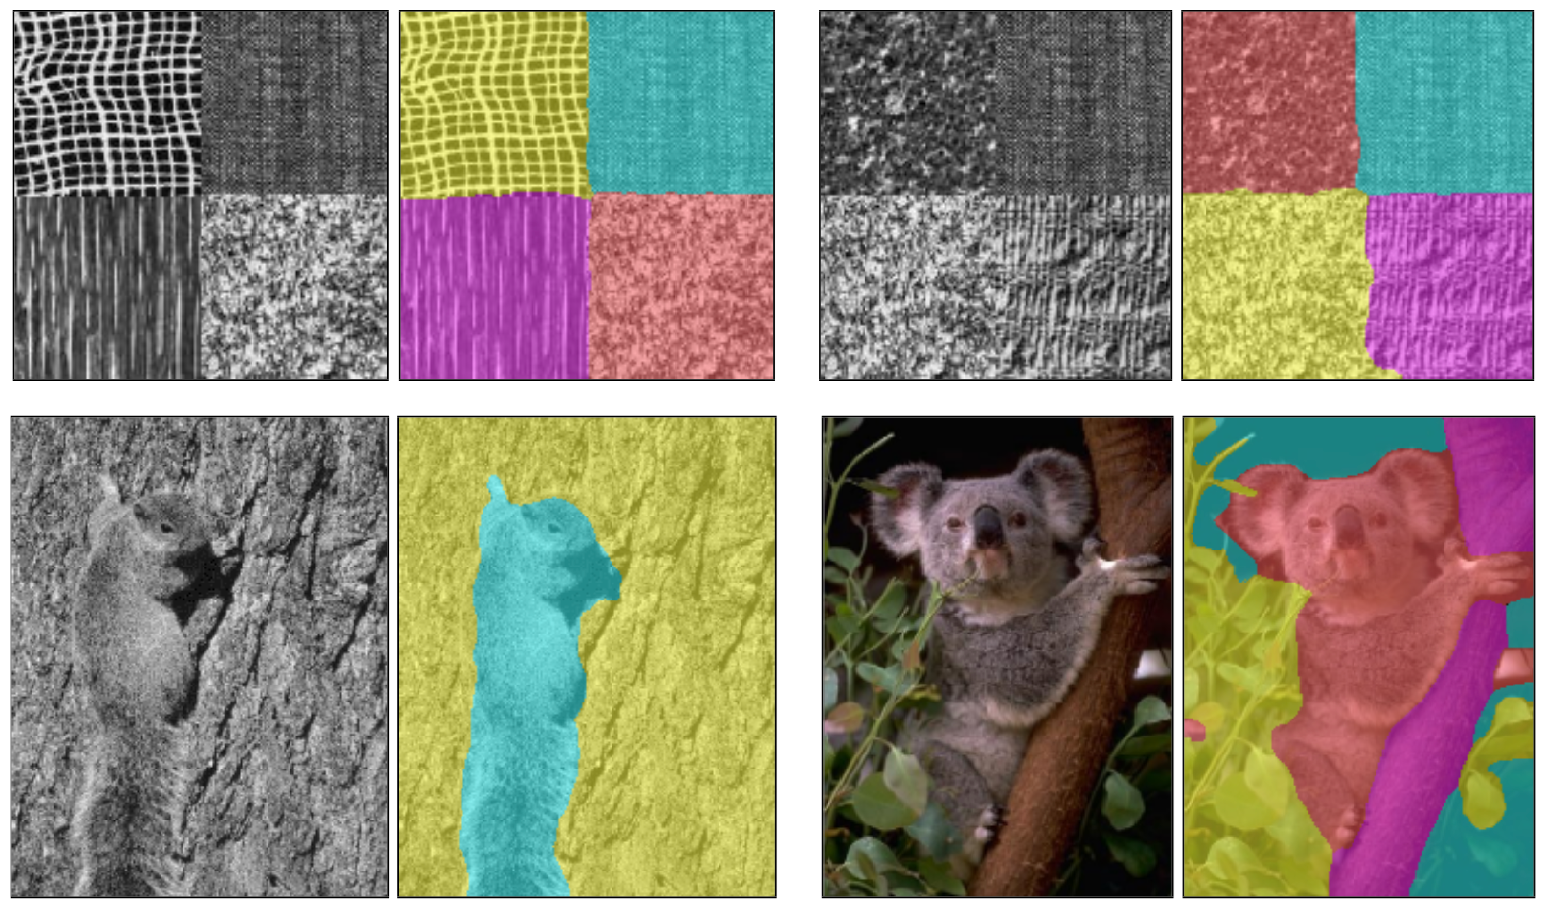
\includegraphics[width=0.45\textwidth]{images/honorable-mentions-1-2-combined.png}
    \caption{\textbf{Top:} Segmentation of two artificial texture images. \textbf{Bottom} Segmentation of color images \cite{Brox2004}.}
    \label{fig:honorable-mentions-1-2-combined}
\end{figure}

\begin{figure}[!t]
    \centering
    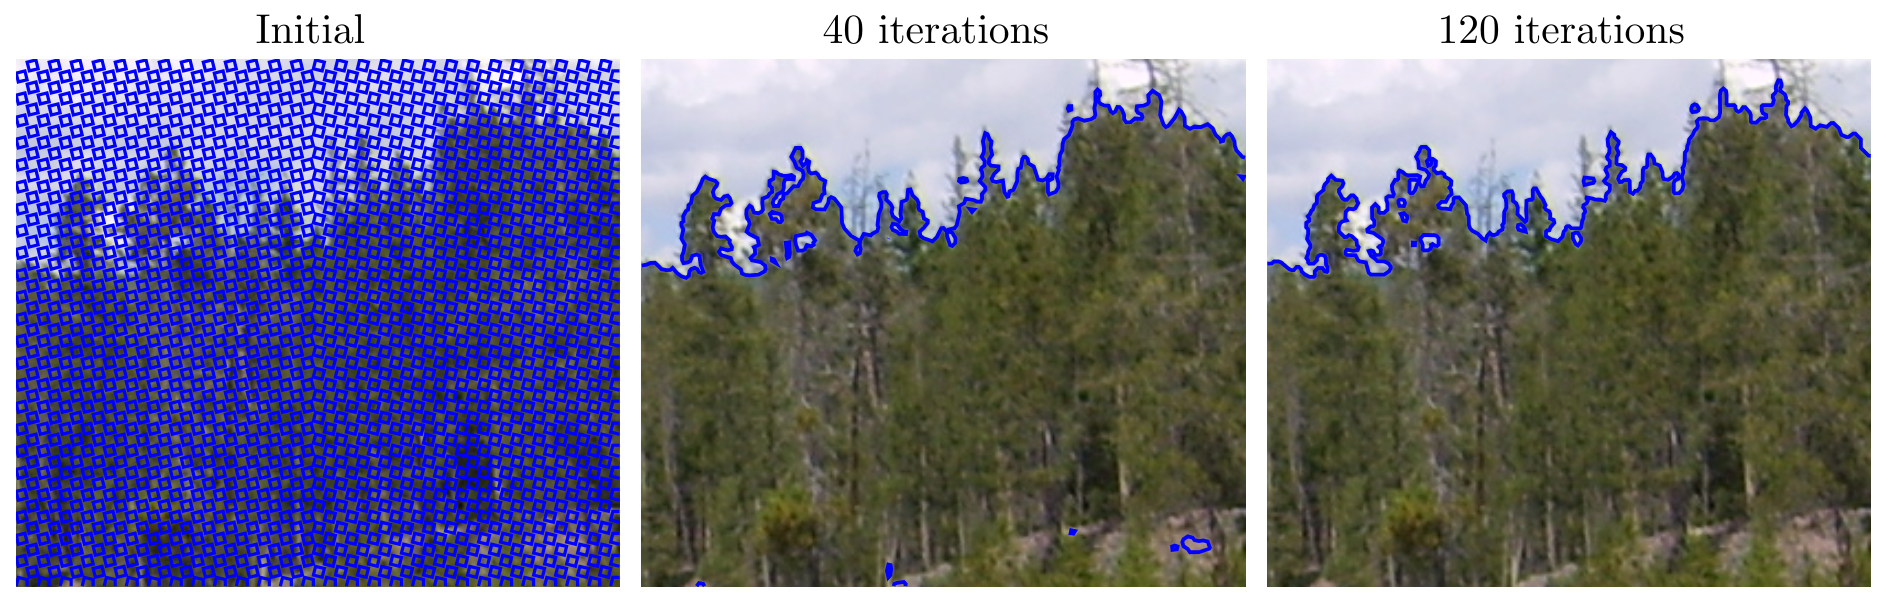
\includegraphics[width=0.5\textwidth]{images/honorable-mentions-7.png}
    \caption{The Chan--Sandberg--Vese (2000) \cite{Chan2000} method can be used to segment color images \cite{getreuer}.}
    \label{fig:honorable-mentions-7}
\end{figure}

\begin{figure}[!t]
    \centering
    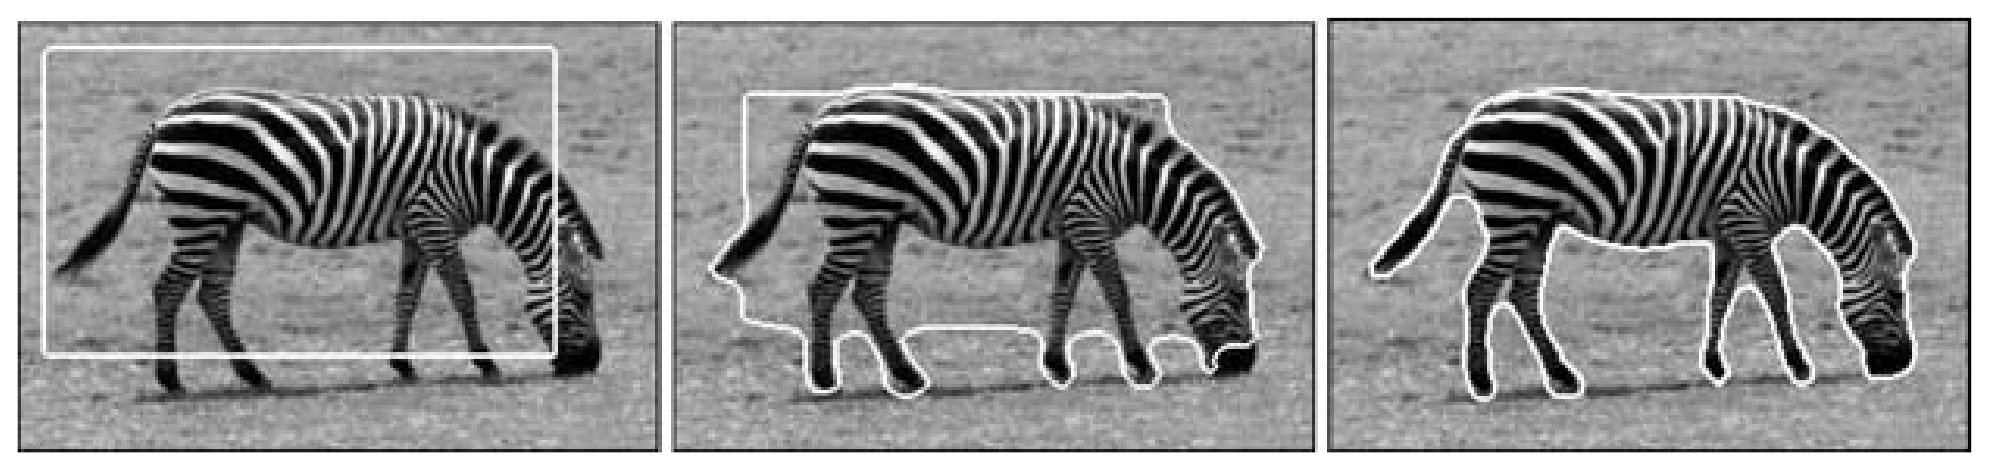
\includegraphics[width=0.5\textwidth]{images/honorable-mentions-5.png}
    \caption{Curve evolution for the segmentation of a zebra image. Here, a rectangle is used as initialization but small circles also lead to a similar result \cite{Cremers2006}.}
    \label{fig:honorable-mentions-5}
\end{figure}

\begin{figure}[!t]
    \centering
    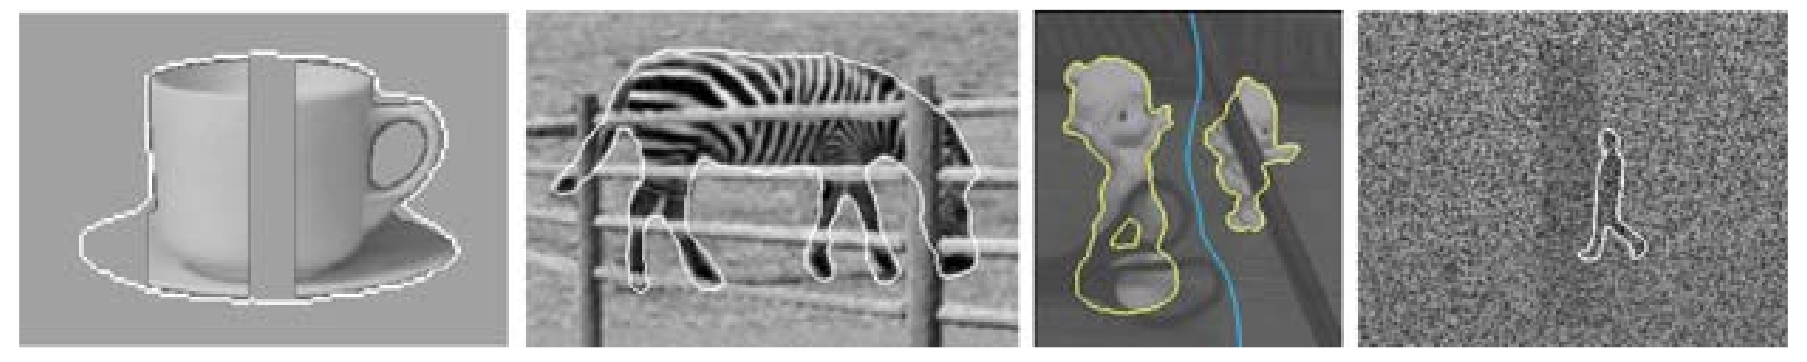
\includegraphics[width=0.5\textwidth]{images/honorable-mentions-6.png}
    \caption{Sample segmentations using statistical shape priors. From left to right, the shape priors are a single static shape prior, uniformly distributed in the PCA subspace, automatically selected from multiple shape instances \cite{Cremers2006}.}
    \label{fig:honorable-mentions-6}
\end{figure}

\section{Conclusion}
T. Chan and L. Vese (2001) introduced an active contour model, that does not rely on gradient computation, based on the \emph{Mumford--Shah functional} \cite{MumfordShah} and the level set method \cite{Osher1988}, is robust to noise, does and is capable of detecting objects with non-gradient and smooth boundaries. Furthermore, it efficiently identifies interior contours with a single flexible initial curve, which does not need to encircle the target objects.

In conclusion, the Chan--Vese model represented a significant breakthrough in image segmentation, which laid the groundwork for more advanced image segmentation techniques, despite its limitations briefly touched in Sec. \ref{sec:limitations-of-the-model}. Its legacy is evident in its widespread adoption and the continuous exploration of its potential for addressing complex image analysis challenges.

\balance

\bibliography{my_bibliography}

\end{document}